%--------------------------------------------------------
% 1. 本模板是通过现用现学不断积累修改得到的,其中必有大量不恰当之处,欢迎批评指教。
% 2. 本模板适合于毕业论文答辩、课程大作业展示等内容比较少的场景。幻灯片上方导航栏虽然能明显区别Beamer和PPT,在文档较短时属于加分项,但在太长时显得累赘。
% 3. 本模板不局限于中国科学技术大学使用,只用修改.sty文件中变量ustcblue的rgb参数就可以改变颜色风格,替换111.png和112.png两个图片就可以修改背景。 
% 4. background文件夹中包含了两个背景图片的.png格式和.psd格式,其中.psd格式可以自由修改。
% 5. 本模板在参考了很多优秀的模板和论坛上的回答,如https://www.latexstudio.net/archives/51752.html, https://github.com/teancake/latex-beamer-beihang, https://tex.stackexchange.com/questions/167648/beamer-navigation-symbols-inside-footline 等等,非常感谢。
%--------------------------------------------------------
%--------------------------------------------------------
% 注意:
% 1. 请设置XeLaTeX编译否则可能无法生成PDF;修改很简单,可自行百度。
% 2. 文档推荐使用微软雅黑字体,若使用overleaf等请自行适配微软雅黑或更改成其他字体。
% 3. 需要使用新功能时,可以修改或添加引用的包。
%--------------------------------------------------------
\documentclass{beamer}%[hyperref,UTF8,11pt]
\usepackage{ctex}
\usepackage[utf8]{inputenc}
\setbeamersize{text margin left=0.042\paperwidth,text margin right=0.042\paperwidth}% 调整左右边距

\usepackage{fontspec}
\usepackage{comment}
\usepackage{xeCJK}
\usepackage{hyperref}
\usepackage{graphicx}
\usepackage{epstopdf}
\usepackage{bm}

\usepackage{array} 
\usepackage{cases}
\usepackage{multirow} 
\usepackage{enumerate}
\usepackage{algorithm}
\usepackage{algorithmic}
\usepackage{xcolor}
\usepackage{amsmath, amsfonts, amssymb} % math equations, symbols
\usepackage[english]{babel}
\usepackage{color}      % color content
\usepackage{graphicx}   % import figures
\usepackage{url}        % hyperlinks
\usepackage{bm}         % bold type for equations
\usepackage{multirow}
\usepackage{booktabs}
\usepackage{epstopdf}
\usepackage{epsfig}
\usepackage{algorithm}
\usepackage{algorithmic}
\hypersetup{CJKbookmarks=true}
\usepackage{url}
\usepackage{amsmath}
\usepackage{amsthm}
\newtheorem{assumption}{假设}
\newtheorem{proposition}{性质}
\usepackage{booktabs} 
\usepackage[backend=biber,style=numeric,sorting=none]{biblatex}
\beamertemplatetextbibitems

\setcounter{tocdepth}{1}
\usepackage{subcaption}
\usepackage{amsmath}

\usepackage{ustcbeamersx}
\graphicspath{{image/} {background/}}


\setsansfont{Microsoft YaHei} % 一般建议是微软雅黑,可以修改成其他字体。
\setCJKmainfont{Microsoft YaHei}
%\setCJKmainfont{SimHei}
\usefonttheme{professionalfonts}


\usepackage[UTF8,noindent]{ctexcap}  %使用中文输入及显示


% 第一页的设置
\title[硕士论文答辩]{\zihao{3} \kaishu 基于机器学习的无人机xxx方法研究}% 方括号内容显示在页脚,花括号内容是全称

\author{\noindent 汤姆}
\institute[HEU]
{   

	\noindent 导师:风二中教授\\
	
	\medskip
	\noindent \textit{ tonixtom@hrbeu.edu.cn} 
}
\date{\today} % Date, can be changed to a custom date


%
%\AtBeginSection[]% 每章之前加目录,不喜欢可以注释掉
%{
%	\begin{frame}{目录}
%		\transfade%淡入淡出效果
%		\tableofcontents[sectionstyle=show/shaded,subsectionstyle=show/shaded/hide] %突出显示当前章节,而其它章节都进行了淡化处理
%		\addtocounter{framenumber}{-1}  %目录页不计算页码
%	\end{frame}
%}


\begin{document}
	\begin{frame}
		\pgfdeclareimage[width=\paperwidth,height=0.9575\paperheight]{bg}{./background/background1.png}
		%\transfade 渐变
		\titlepage % Print the title page as the first slide
	\end{frame}
	
%%\section{目录}
%	\begin{frame}{目录}
%		\pgfdeclareimage[width=\paperwidth,height=0.9575\paperheight]{bg}{112.png}
%		%\transfade
%		\onslide<1->条目;
%		
%		\onslide<2->条目:
%		\begin{itemize}
%			\item<3-> 条目;
%			\item<4-> 条目;
%		\end{itemize}
%		%	\end{itemize}
%	\end{frame}
	
	\begin{frame}{目录}  % 总的目录页 可以注释掉
		\pgfdeclareimage[width=\paperwidth,height=0.9575\paperheight]{bg}{./background/background2.png}
		%[width=\paperwidth,height=0.9575\paperheight]{bg}{112.png}
		%\transfade%淡入淡出 
		\tableofcontents 
	\end{frame}		
	
	
	\section{绪论}
	   \begin{frame}{图}
		\begin{columns}[T] % align columns
			\begin{column}<0->{.65\textwidth}
				\begin{itemize}
					\item<1-> 128
						\begin{itemize}
							\item<1->123 
							\item<1-> 123
						\end{itemize}
					\item<2-> 122
						\begin{itemize}	
							\item<2-> 129
						\end{itemize}
				\end{itemize}
			\end{column}%			
			\hfill%	
			\begin{column}<0->{.40\textwidth}
				\begin{figure}[thpb]
					\centering
					\resizebox{1\linewidth}{!}{
							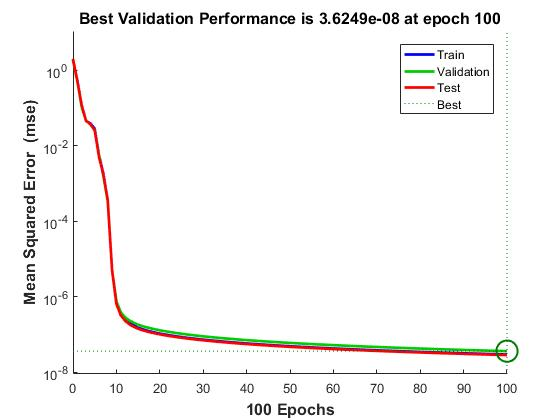
\includegraphics{temp.jpg}
					}
					%\includegraphics[scale=1.0]{figurefile}
					%\caption{}
					\label{fig:campus}
				\end{figure}
			\end{column}%
		\end{columns}
	\end{frame}
	
	   \begin{frame}{图}
		\begin{figure}[htb]
			%  \centering
			\label{fig:example}
			\begin{subfigure}{.45\textwidth}
				\centering
				
\includegraphics[width=\textwidth]{badge.jpeg}
				\caption{校徽}
				\label{fig:logoa}
			\end{subfigure}
			\begin{subfigure}{.45\textwidth}
				\centering
				
\includegraphics[width=\textwidth]{badge.jpeg}
				\caption{校徽}
				\label{fig:logob}
			\end{subfigure}
			\caption{校徽}
			%\note{注:}
		\end{figure}
	\end{frame}
	
	
	\section{机器学习相关技术}
	\begin{frame}{表格}
		\footnotesize
		\begin{table}[htb]
			\setlength{\abovecaptionskip}{-1mm} 
		%	\setlength{\belowcaptionskip}{-2.3mm}
			\centering
			\caption{三线表}
			\label{tab:err1}
			%\resizebox{\textwidth}{19mm}{ %用于控制表格宽度
				\begin{tabular}{ccccccccc}
					\toprule
					\text{模型}&\text{组别}  & $D_0$ & $D_1$  & $D_2$                    \\
					\midrule
					1&(1.1) & 0.0600&	0.0600&	0.0800  \\
					&(1.2) & 0.0600&	0.0600&	0.0800  \\
					2&(2.1) & 0.0600&	0.0600&	0.0800  \\
					&(2.2) & 0.0600&	0.0600&	0.0800  \\
					\bottomrule
			\end{tabular}%}
			%  \note{注:} %可以调整字体
		\end{table}
	
	\begin{table}[H]
		\centering
		\caption{The relationship between $f$ and $f'$.}
		\def\arraystretch{1.5}
		\begin{tabular}{|l|p{3in}|}
			\hline
			$f(x)$ & $f'(x)$ \\ \hline
			$x>0$ & The function $f(x)$ is increasing. The function $f(x)$ is increasing. The function $f(x)$ is increasing. The function $f(x)$ is increasing. The function $f(x)$ is increasing. \\ \hline
		\end{tabular}
	\end{table}
		
	\end{frame}


    \section{机器学习模型}
\begin{frame}{表格}

\begin{table}[H]
	\centering
	\def\arraystretch{1.5}
	\begin{tabular}{|c||c|c|c|c|c|}
		\hline
		$x$ & 1 & 2 & 3 & 4 & 5 \\ \hline
		$f(x)$ & $\frac{1}{2}$ & 11 & 12 & 13 & 14 \\ \hline
	\end{tabular}
	\caption{These values represent the function $f(x)$.}
\end{table}


\begin{table}[H]
	\centering
	\caption{The relationship between $f$ and $f'$.}
	\def\arraystretch{1.5}
	\begin{tabular}{|l|p{3in}|}
		\hline
		$f(x)$ & $f'(x)$ \\ \hline
		$x>0$ & The function $f(x)$ is increasing. The function $f(x)$ is increasing. The function $f(x)$ is increasing. The function $f(x)$ is increasing. The function $f(x)$ is increasing. \\ \hline
	\end{tabular}
\end{table}

\end{frame}
	
	\section{实验与仿真}
	\begin{frame}{定理}
		\begin{theorem}[勾股定理]
			勾三股四弦五。
		\end{theorem}
	证明:
	xxx,证毕。
	
	$\hfill\qedsymbol$
	
	The function $f(x)=(x-3)^2+\frac{1}{2}$ has domain $\mathrm{D}_f:(-\infty,\infty)$ and range $\mathrm{R}_f:\left[\frac{1}{2},\infty\right)$.\\

	$\displaystyle{\lim \limits_{x \to a} \frac{f(x)-f(a)}{x-a}=f'(a)}$\\
	
	$\displaystyle{\int_a^b f(x) \,dx=\lim \limits_{x \to \infty} \sum \limits_{k=1}^{n} f(x_k) \cdot \Delta x}$\\
	
	$\vec{v}=v_1 \vec{i}+v_2 \vec{j}=\langle v_1, v_2 \rangle$
	\end{frame}

    \section{总结}
	\begin{frame}
		\frametitle{总结}	
		
		\begin{align}
			5x^2-9=x+3\\
			5x^2-x-12=0
		\end{align}
		
		
		\begin{align}
			5x^2-9=x+3\\
			5x^2-x-12=0
		\end{align}
	\end{frame}

	
	
	
	\begin{frame}
			\pgfdeclareimage[width=\paperwidth,height=0.9575\paperheight]{bg}{./background/background3.png}
		\frametitle{ \kaishu\textbf{ 致谢}}
		\centerline{\Huge \youyuan 请各位老师批评指正}
	\end{frame}
	
	
	
\end{document}